\definecolor{warningbackground}{RGB}{252,226,158}
%\definecolor{infoforeground}{RGB}{58,135,173}
\definecolor{warningborder}{RGB}{219,194,129}
\definecolor{link}{RGB}{51,102,204}

\usepackage{environ}
\usepackage{tikz}
\usetikzlibrary{fit,backgrounds,calc}

\NewEnviron{warning}
{
    \vskip \baselineskip
    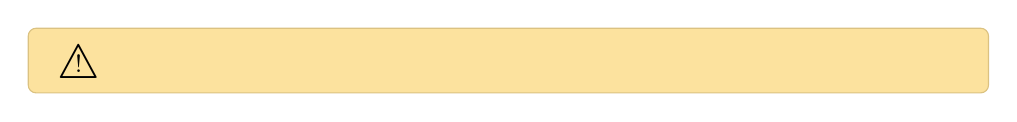
\begin{tikzpicture}
        \node[inner sep=1pt, draw=warningborder, rounded corners=0.1cm, fill=warningbackground] (box) {
            \parbox[t]{\textwidth}
            {%
                \begin{minipage}{.1\textwidth}
                    \vskip 4pt
                    \centering\tikz[scale=1]
                    \node[scale=1]
                    {
                        \makebox[0pt][c]{%
                        \makebox[0pt][c]{\raisebox{.2em}{\small!}}%
                        \makebox[0pt][c]{\LARGE$\bigtriangleup$}}
                    };
                \end{minipage}%
                \begin{minipage}{.85\textwidth}
                    \vspace{5pt}
                    \BODY
                    \vspace{5pt}
                \end{minipage}\hfill
            }%
        };
    \end{tikzpicture}
}

\usepackage[colorlinks=true, linkcolor=link, urlcolor=link, citecolor=link, anchorcolor=link]{hyperref}
%\usepackage{color}
%\renewcommand\UrlFont{\color{blue}\rmfamily}
\newcommand{\secref}[1]{\hyperref[#1]{Abschnitt~\ref{#1}}}
\newcommand{\figref}[1]{\hyperref[#1]{Abbildung~\ref{#1}}}
\newcommand{\tabref}[1]{\hyperref[#1]{Tabelle~\ref{#1}}}